\documentclass[10pt,a4paper]{article}
\usepackage[margin=.5in]{geometry}
\usepackage[utf8]{inputenc}
\usepackage[T1]{fontenc}
\usepackage{dot2texi}
\usepackage{tikz}
\usetikzlibrary{shapes,arrows}\usepackage{amsmath}
\usepackage{amsfonts}
\usepackage{amssymb}
\usepackage{graphicx}
\usepackage{verbatim}
\usepackage{listings}
\usepackage{color}
\usepackage{parskip}
\usepackage{float}
\usepackage{mathtools}
% \usepackage{minted}
\usepackage{verbatim}
\usepackage{listings}
\usepackage{optidef}
\usepackage{bm}
\usepackage{algorithm}
\usepackage{algpseudocode}
\usepackage{hyperref}
\usepackage{cleveref}
\usepackage{enumerate}
\usepackage{caption}
\usepackage{subcaption}
\restylefloat{figure}
% \setminted{fontsize=\tiny,linenos=true,frame=single,breaklines=true}
\allowdisplaybreaks

\algrenewcommand{\Return}{\State\algorithmicreturn~}
\DeclareMathOperator*{\argmin}{arg\,min}

\title{IPM forumalations}
\author{Pratyai Mazumder}

\renewcommand{\thesubsection}{\thesection.\roman{subsection}}
\newcommand{\R}{\mathbb{R}}
\newcommand{\Rgz}{\R_{>0}}
\newcommand{\Rgez}{\R_{\geq0}}
\newcommand{\Rlz}{\R_{<0}}
\newcommand{\Rlez}{\R_{\leq0}}
\newcommand{\Oo}{\mathcal{O}}

\begin{document}

\maketitle

\tableofcontents

\section{Original Problem}

\subsection{Primal}

\begin{mini}|s|
{\mathbf{x}}{\mathbf{c}^T\mathbf{x}}{}{}
\addConstraint{\mathbf{A}\mathbf{x}}{= \mathbf{b}}
\addConstraint{\mathbf{x}}{\leq \bm{u}}
\addConstraint{\mathbf{x}}{\in \Rgez^m}
\end{mini}

\subsection{Primal Standard Form}

\begin{mini}|s|
{\mathbf{x}}{\mathbf{c}^T\mathbf{x}}{}{}
\addConstraint{\mathbf{A}\mathbf{x}}{= \mathbf{b}}
\addConstraint{\mathbf{x} + \mathbf{x}_u}{= \bm{u}}
\addConstraint{\mathbf{x}, \mathbf{x}_u}{\in \Rgez^m, \Rgez^m}
\end{mini}

\subsection{Dual}

\begin{maxi}|s|
{\mathbf{y}, \mathbf{y}_u}{\mathbf{b}^T\mathbf{y} + \mathbf{u}^T\mathbf{y}_u}{}{}
\addConstraint{\mathbf{A}^T\mathbf{y} + \mathbf{y}_u}{\leq \mathbf{c}}
\addConstraint{\mathbf{y}, \mathbf{y}_u}{\in \R^n, \Rgez^m}
\end{maxi}

\subsection{Dual Standard form}

\begin{maxi}|s|
{\mathbf{y}, \mathbf{y}_u}{\mathbf{b}^T\mathbf{y} + \mathbf{u}^T\mathbf{y}_u}{}{}
\addConstraint{\mathbf{A}^T\mathbf{y} + \mathbf{y}_u + \mathbf{z}}{= \mathbf{c}}
\addConstraint{\mathbf{y}, \mathbf{y}_u, \mathbf{z}}{\in \R^n, \Rgez^m, \Rgez^m}
\end{maxi}

But if we want $\mathbf{y}$ variables to be free, then dualize the standard from, then standardize again:
\begin{maxi}|s|
{\mathbf{y}, \mathbf{y}_u}{\mathbf{b}^T\mathbf{y} + \mathbf{u}^T\mathbf{y}_u}{}{}
\addConstraint{\mathbf{A}^T\mathbf{y} + \mathbf{y}_u + \mathbf{z}_1}{= \mathbf{c}}
\addConstraint{\mathbf{y}_u + \mathbf{z}_2}{= \bm{0}}
\addConstraint{\mathbf{y}, \mathbf{y}_u, \mathbf{z}_1, \mathbf{z}_2}{\in \R^n, \R^m, \Rgez^m, \Rgez^m}
\end{maxi}

\section{Solver Forms}

\subsection{Long Step Path Following Method}

Ref: \href{https://link.springer.com/book/10.1007/978-0-387-40065-5}{Numerical Optimization (Alg. 14.2)}

It turns out that staying inside the \emph{good neighbourhood} of the central path can be difficult with an approximate solver. So, we will use \texttt{Mehrotra's Predictor Corrector Method} to solve the sample problems. The formulation is the same in both cases, so we will describe it here for simplicity.

Due to the formulation, we have to work with the standard form.

\subsubsection{Primal}

\begin{mini}|s|
{}{c^Tx}{}{}
\addConstraint{Ax}{= b}
\addConstraint{x}{\in \Rgez^n}
\end{mini}

$$A = \begin{bmatrix}\mathbf{A} & \bm{0} \\ \mathbf{I} & \mathbf{I}\end{bmatrix} ~~~|~~~ x = \begin{bmatrix}\mathbf{x} \\ \mathbf{x}_u\end{bmatrix} ~~~|~~~ b = \begin{bmatrix}\mathbf{b} \\ \mathbf{u}\end{bmatrix} ~~~|~~~ c = \begin{bmatrix}\mathbf{c} \\ \bm{0}\end{bmatrix}$$

\subsubsection{Dual}

\begin{maxi}|s|
{}{b^Ty}{}{}
\addConstraint{A^T\lambda + s}{= c}
\addConstraint{\lambda, s}{\in \R^m, \Rgez^n}
\end{maxi}

$$A = \begin{bmatrix}\mathbf{A} & \bm{0} \\ \mathbf{I} & \mathbf{I}\end{bmatrix} ~~~|~~~ \lambda = \begin{bmatrix}\mathbf{y} \\ \mathbf{y}_u\end{bmatrix} ~~~|~~~ b = \begin{bmatrix}\mathbf{b} \\ \mathbf{u}\end{bmatrix} ~~~|~~~ c = \begin{bmatrix}\mathbf{c} \\ \bm{0}\end{bmatrix} ~~~|~~~ s = \begin{bmatrix}\mathbf{z}_1 \\ \mathbf{z}_2\end{bmatrix} = \begin{bmatrix}\mathbf{s} \\ \mathbf{s}_u\end{bmatrix}$$

\subsubsection{Big KKT}

$$\begin{bmatrix}
0 & A^T & I \\
A & 0 & 0 \\
S & 0 & X
\end{bmatrix}
\begin{bmatrix}\delta_x \\ \delta_y \\ \delta_s\end{bmatrix} = 
\begin{bmatrix}-r_d \\ -r_p \\ -r_c\end{bmatrix}$$

\subsubsection{Small KKT}

$$\begin{bmatrix}-X^{-1}S & A^T \\ A & 0\end{bmatrix}
\begin{bmatrix}\delta_x \\ \delta_y\end{bmatrix} = 
\begin{bmatrix}-r_d + X^{-1}r_c \\ -r_p\end{bmatrix}$$
$$\delta_s = -X^{-1}(r_c + Sd_x)$$

\subsubsection{No KKT}

Let $M := AS^{-1}XA^T$ (note: this is \emph{not necessarily} a Laplacian). Then,
\begin{align*}
\delta_y &= M^+(-r_p - AS^{-1}Xr_d + AS^{-1}r_c) \\
\delta_x &= -S^{-1}(r_c - X(r_d + A^Td-y))\\
\delta_s &= -X^{-1}(r_c + Sd_x)
\end{align*}
Observe that solving the $Md_y = -r_p - AS^{-1}Xr_d + AS^{-1}r_c$ system is difficult --- even a fast Laplacian solver cannot directly help. The other inversions of diagonal matrices and multiplications with sparse or diagonal matrices can be done relatively easily (i.e. $\Oo(nnz)$).

\subsubsection{Approximate KKT}

Substituting in the $Md_y = -r_p - AS^{-1}Xr_d + AS^{-1}r_c = -r_p -  AS^{-1}(Xr_d - r_c)$ system:
\begin{align*}
\begin{bmatrix}\mathbf{A} & 0 \\ I & I\end{bmatrix}
\begin{bmatrix}\mathbf{S}^{-1} & 0 \\ 0 & \mathbf{S}_u^{-1}\end{bmatrix}
\begin{bmatrix}\mathbf{X} & 0 \\ 0 & \mathbf{X}_u\end{bmatrix}
\begin{bmatrix}\mathbf{A}^T & I \\ 0 & I\end{bmatrix}
\begin{bmatrix}d_y \\ d_{yu}\end{bmatrix} &=
-\begin{bmatrix}r_p \\ r_{pu}\end{bmatrix}
- \begin{bmatrix}\mathbf{A} & 0 \\ I & I\end{bmatrix}
\begin{bmatrix}\mathbf{S}^{-1} & 0 \\ 0 & \mathbf{S}_u^{-1}\end{bmatrix}
\Big(
	\begin{bmatrix}\mathbf{X} & 0 \\ 0 & \mathbf{X}_u\end{bmatrix}
	\begin{bmatrix}r_d \\ r_{du}\end{bmatrix}
	+ \begin{bmatrix}r_c \\ r_{cu}\end{bmatrix}
\Big) \\
\intertext{Simplifying:}
\begin{bmatrix}
	\mathbf{A}\mathbf{S}^{-1}\mathbf{X}\mathbf{A}^T & \mathbf{A}\mathbf{S}^{-1}\mathbf{X} \\
	\mathbf{S}^{-1}\mathbf{X}\mathbf{A}^T & \mathbf{S}^{-1}\mathbf{X}+\mathbf{S}_u^{-1}\mathbf{X}_u
\end{bmatrix}
\begin{bmatrix}d_y \\ d_{yu}\end{bmatrix} &=
\begin{bmatrix}
	-r_p - \mathbf{A}\mathbf{S}^{-1}(\mathbf{X}r_d - r_c) \\
	-r_{pu} - \mathbf{S}^{-1}(\mathbf{X}r_d - r_c) - \mathbf{S}_u^{-1}(\mathbf{X}_ur_{du} - r_{cu})
\end{bmatrix} \\
\intertext{Let $\mathbf{K} := \mathbf{S}^{-1}\mathbf{X}+\mathbf{S}_u^{-1}\mathbf{X}_u$ and $r_q := -r_{pu} - \mathbf{S}^{-1}(\mathbf{X}r_d - r_c) - \mathbf{S}_u^{-1}(\mathbf{X}_ur_{du} - r_{cu})$:}
\begin{bmatrix}
	\mathbf{A}\mathbf{S}^{-1}\mathbf{X}\mathbf{A}^T & \mathbf{A}\mathbf{S}^{-1}\mathbf{X} \\
	\mathbf{S}^{-1}\mathbf{X}\mathbf{A}^T & \mathbf{K}
\end{bmatrix}
\begin{bmatrix}d_y \\ d_{yu}\end{bmatrix} &=
\begin{bmatrix}
	-r_p - \mathbf{A}\mathbf{S}^{-1}(\mathbf{X}r_d - r_c) \\
	r_q
\end{bmatrix} \\
\intertext{Observing that $\mathbf{K}$ is invertible, and scaling:}
\begin{bmatrix}
	\mathbf{A}\mathbf{S}^{-1}\mathbf{X}\mathbf{A}^T & \mathbf{A}\mathbf{S}^{-1}\mathbf{X} \\
	\mathbf{K}^{-1}\mathbf{S}^{-1}\mathbf{X}\mathbf{A}^T & I
\end{bmatrix}
\begin{bmatrix}d_y \\ d_{yu}\end{bmatrix} &=
\begin{bmatrix}
	-r_p - \mathbf{A}\mathbf{S}^{-1}(\mathbf{X}r_d - r_c) \\
	\mathbf{K}^{-1}r_q
\end{bmatrix} \\
\intertext{Eliminating $d_{yu}$:}
\begin{bmatrix}
	\mathbf{A}(\mathbf{S}^{-1}\mathbf{X} - \mathbf{S}^{-1}\mathbf{X}\mathbf{K}^{-1}\mathbf{S}^{-1}\mathbf{X})\mathbf{A}^T & 0 \\
	\mathbf{K}^{-1}\mathbf{S}^{-1}\mathbf{X}\mathbf{A}^T & I
\end{bmatrix}
\begin{bmatrix}d_y \\ d_{yu}\end{bmatrix} &=
\begin{bmatrix}
	-r_p - \mathbf{A}\mathbf{S}^{-1}(\mathbf{X}r_d - r_c + \mathbf{X}\mathbf{K}^{-1}r_q) \\
	\mathbf{K}^{-1}r_q
\end{bmatrix} \\
\intertext{Let $\mathbf{D} := \mathbf{S}^{-1}\mathbf{X} - \mathbf{S}^{-1}\mathbf{X}\mathbf{K}^{-1}\mathbf{S}^{-1}\mathbf{X} = \mathbf{S}^{-1}\mathbf{X}(I - \mathbf{K}^{-1}\mathbf{S}^{-1}\mathbf{X})$ and $\mathbf{L} := \mathbf{A}\mathbf{D}\mathbf{A}^T$ and $r_s := -r_p - \mathbf{A}\mathbf{S}^{-1}(\mathbf{X}r_d - r_c + \mathbf{X}\mathbf{K}^{-1}r_q)$:}
\begin{bmatrix}
	\mathbf{L} & 0 \\
	\mathbf{K}^{-1}\mathbf{S}^{-1}\mathbf{X}\mathbf{A}^T & I
\end{bmatrix}
\begin{bmatrix}d_y \\ d_{yu}\end{bmatrix} &=
\begin{bmatrix}
	r_s \\
	\mathbf{K}^{-1}r_q
\end{bmatrix} \\
\intertext{Pretending that $\mathbf{L}$ is invertible:}
\begin{bmatrix}
	I & 0 \\
	\mathbf{K}^{-1}\mathbf{S}^{-1}\mathbf{X}\mathbf{A}^T & I
\end{bmatrix}
\begin{bmatrix}d_y \\ d_{yu}\end{bmatrix} &=
\begin{bmatrix}
	\mathbf{L}^{-1}r_s \\
	\mathbf{K}^{-1}r_q
\end{bmatrix} \\
\intertext{Eliminating $d_y$,}
\delta_y = \begin{bmatrix}
	I & 0 \\
	0 & I
\end{bmatrix}
\begin{bmatrix}d_y \\ d_{yu}\end{bmatrix} &=
\begin{bmatrix}
	\mathbf{L}^{-1}r_s \\
	\mathbf{K}^{-1}(r_q - \mathbf{S}^{-1}\mathbf{X}\mathbf{A}^Td_y)
\end{bmatrix} \\
\intertext{And we can apply the remaining formula from \texttt{No KKT}:}
\delta_x &= -S^{-1}(r_c - X(r_d + A^Td-y))\\
\delta_s &= -X^{-1}(r_c + Sd_x)
\end{align*}

\subsection{Mehrotra's Predictor Corrector Method}

Ref: \href{https://link.springer.com/book/10.1007/978-0-387-40065-5}{Numerical Optimization (Alg. 14.3)}

We reuse the same solver as \texttt{Long Step Path Following Method}, since the left hand side is the same for all systems that we have to solve, and we can simply provide a different right hand side.

\section{Phase 1}

We want to start the actual optimisation somewhere close to the central path, which is quite difficult to construct. So, we solved the same problem with zero cost first, to get close to the analytic centre of the feasible region.

But it turns out, even Phase-1 doesn't work well if we do not start from a feasible flow, which again is difficult to construct. So, we simply added a \emph{star} node with 0 demand, and connected all the other nodes to it with high cost and capacity. Now it is trivial to construct a feasible flow that only routes through this \emph{star} node.

\section{Integral Flow}

Ref: \href{https://arxiv.org/pdf/1507.08139.pdf}{Flow Rounding (Sec. 4)}

For the problems that converge near the optimal, we can \emph{round} them to an integral flow by cancelling the fractional flows in $\Oo(m\log n)$. This was implemented using \emph{link-cut trees}, although I did not verify that the implementation indeed has the claimed time-complexity.

Currently considering: Instead of rounding the flow at the end, it might be possible to round at every iteration of Phase-2 if the primal infeasibility ($\|r_p\|_\infty$) is low enough. I have not analysed the implication of this for the other termination conditions of the IPM.

\section{Results}

Both of the methods described above were implemented in Julia. \texttt{Mehrotra's method} was used to produce the following results. \href{https://github.com/pratyai/ipm}{This public GitHub repository} contains all relevant codes, runtime logs, and plots. We use some of them here to make a few observations.

\begin{itemize}
\item In all cases, Phase-1 converged relatively quickly (e.g., within 20 iterations, even for the largest problem).
\item In all cases, Phase-2 started with low surrogate duality gap ($\mu$), low primal infeasibility ($\|r_p\|_\infty$) and high dual infeasibility ($\|r_d\|_\infty$).
\item For the first half of Phase-2, $\mu$ \emph{increased}, while $\|r_d\|_\infty$ stayed high. Once $\mu$ roughly matched $\|r_d\|_\infty$, only then both started to decrease together. For the converging problems, $\|r_p\|_\infty$ stayed relatively low --- but for the diverging problems, $\|r_p\|_\infty$ shot up around the same time $\mu$ matched $\|r_d\|_\infty$, and never recovered.
\end{itemize}

\begin{figure}[b]
\centering

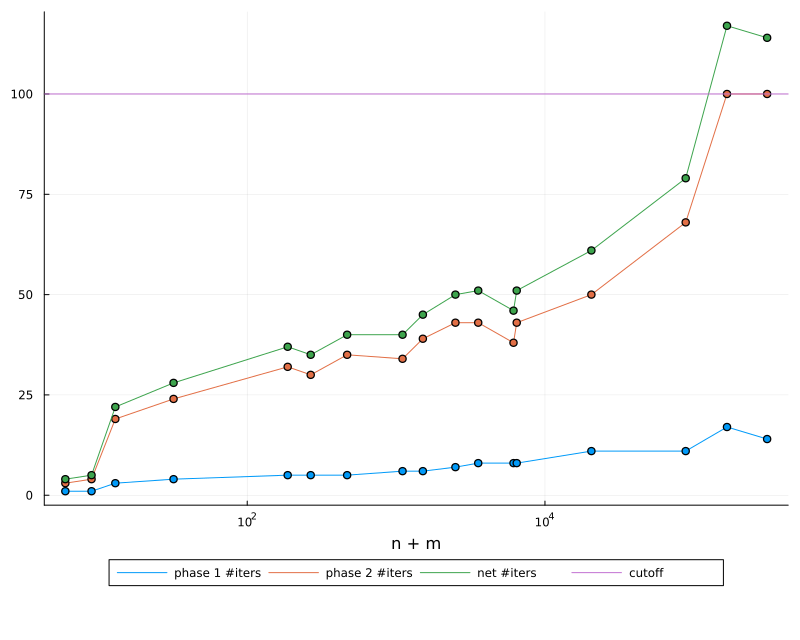
\includegraphics[width=0.7\textwidth]{plots/logs.png}
\caption{Each phase were allowed a maximum of 100 iterations. The two largest problems (\texttt{m = 166088} and \texttt{m = 309364}) diverged. Until then all the problems (up to \texttt{m = 87590}) converged with roughly logarithmic growth of number of iterations with the problem size (i.e., \texttt{n + m})}
\end{figure}

\begin{figure}
\centering

\begin{subfigure}[b]{0.49\textwidth}
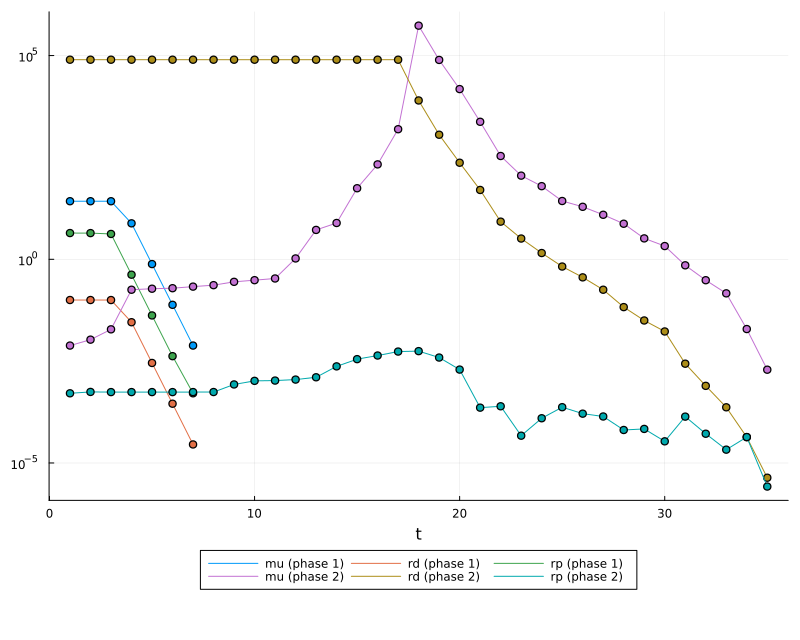
\includegraphics[width=\textwidth]{plots/ng_50_2228_17_5_97.dimacs.log.png}
\caption{\texttt{n = 50, m = 1440}.}
\end{subfigure}
\hfill
\begin{subfigure}[b]{0.49\textwidth}
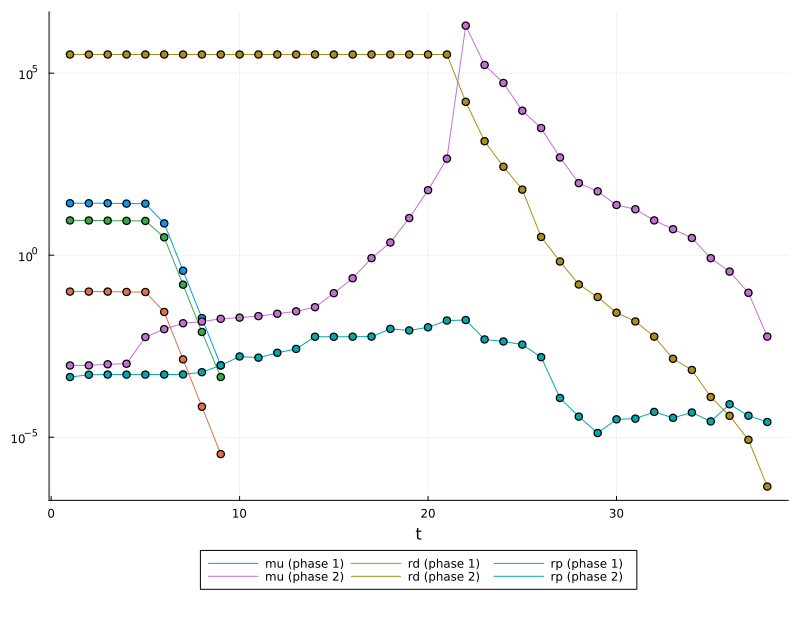
\includegraphics[width=\textwidth]{plots/ng_100_8813_33_9_97.dimacs.log.png}
\caption{\texttt{n = 100, m = 6006}.}
\end{subfigure}

\begin{subfigure}[b]{0.49\textwidth}
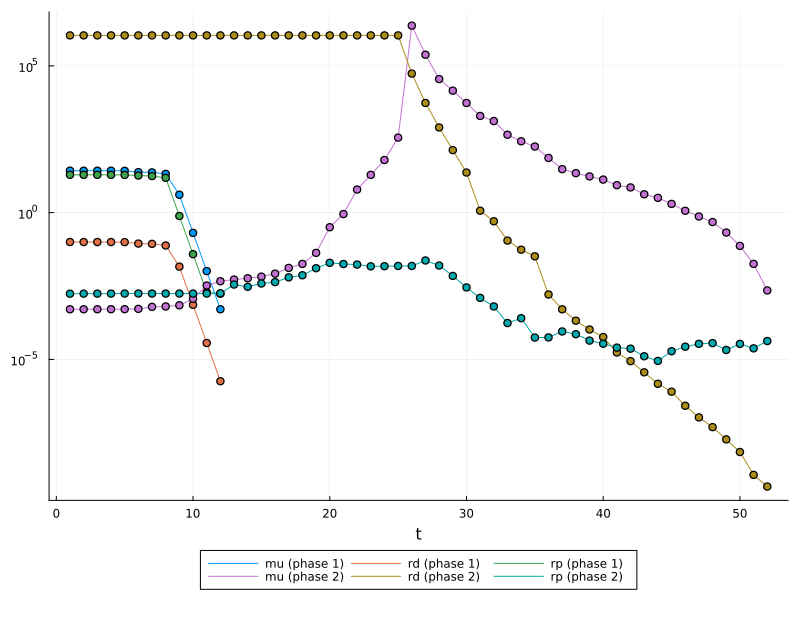
\includegraphics[width=\textwidth]{plots/ng_300_20072_51_84_41.dimacs.log.png}
\caption{\texttt{n = 300, m = 20072}.}
\end{subfigure}
\hfill
\begin{subfigure}[b]{0.49\textwidth}
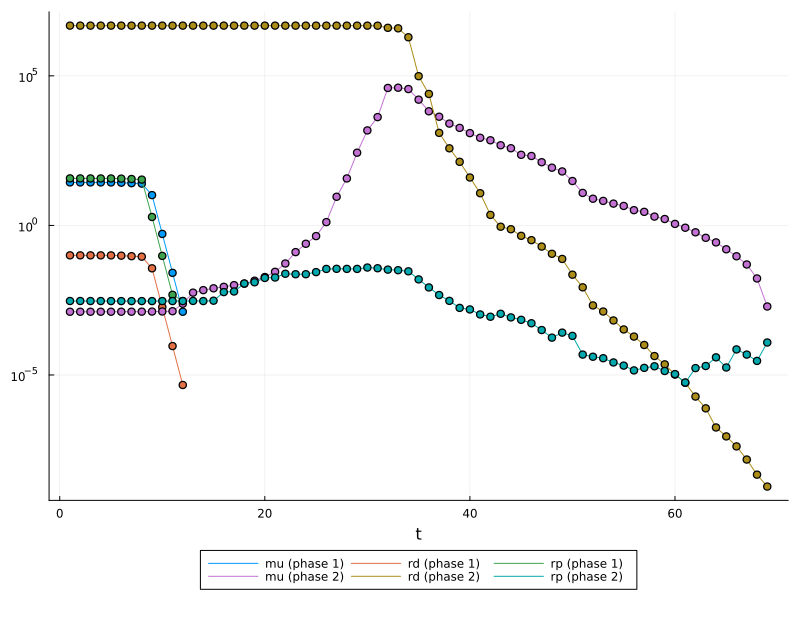
\includegraphics[width=\textwidth]{plots/ng_500_87590_60_43_48.dimacs.log.png}
\caption{\texttt{n = 500, m = 87590}.}
\end{subfigure}

\begin{subfigure}[b]{0.49\textwidth}
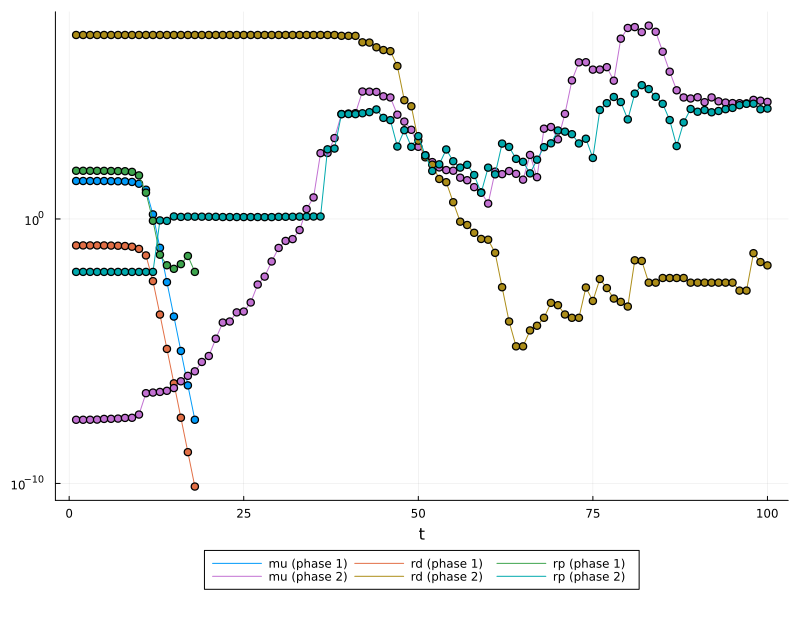
\includegraphics[width=\textwidth]{plots/ng_700_166088_34_286_70.dimacs.log.png}
\caption{\texttt{n = 700, m = 166088}.}
\end{subfigure}
\hfill
\begin{subfigure}[b]{0.49\textwidth}
\includegraphics[width=\textwidth]{plots/ng_1000_309364_236_231_15.dimacs.log.png}
\caption{\texttt{n = 1000, m = 309364}.}
\end{subfigure}

\caption{Progression of surrogate duality gap ($\mu = \frac{s^Tx}{n}$), primal infeasibility ($\|r_p\|_\infty$), and dual infeasibility ($\|r_d\|_\infty$) for some example problems.}
\end{figure}

\end{document}